\documentclass[10pt,a4paper]{article}
\usepackage[utf8]{inputenc}
\usepackage[russian]{babel}
\usepackage{amsmath}
\usepackage{amsfonts}
\usepackage{amssymb}
\usepackage{graphicx}
\usepackage{placeins}
\author{Анастасия Тарасова}
\title{Отчет по лабораторной работе №5\\ Проект OWASP WebGoat}
\begin{document}
\maketitle
\section{Цель работы}
Изучить описание деятельности самых распространенных веб-уязвимостей согласно рейтингу OWASP.
\section{Ход работы}
Запустим уязвимое приложение WebGoat (рисунок 1).
\FloatBarrier
\begin{figure}[h!]
\centering
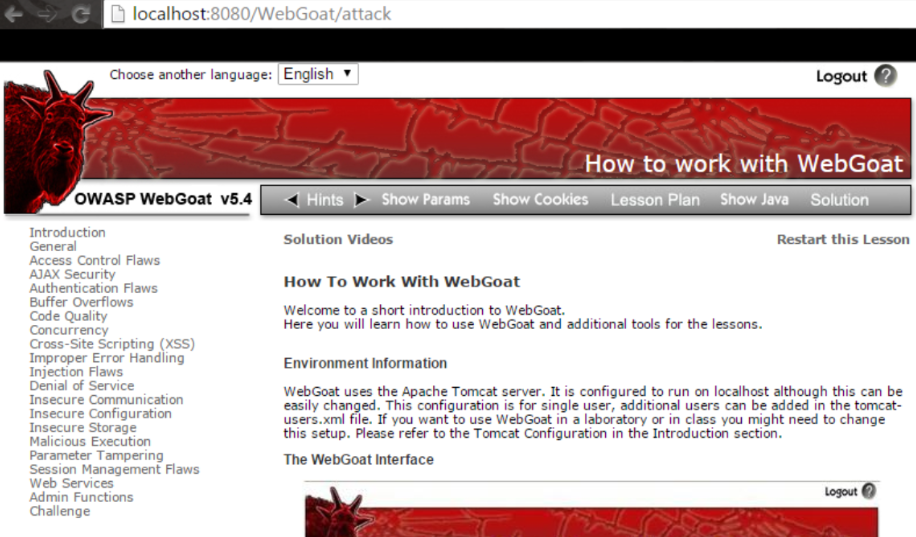
\includegraphics[scale=0.5]{1}
\caption{Запуск WebGoat в браузере Mantra}
\end{figure}
\FloatBarrier
Настроим инструмент Mantra для использования ZAP (сканера безопасновати) в качестве прокси-сервера (рисунок 2).
\FloatBarrier
\begin{figure}[h!]
\centering
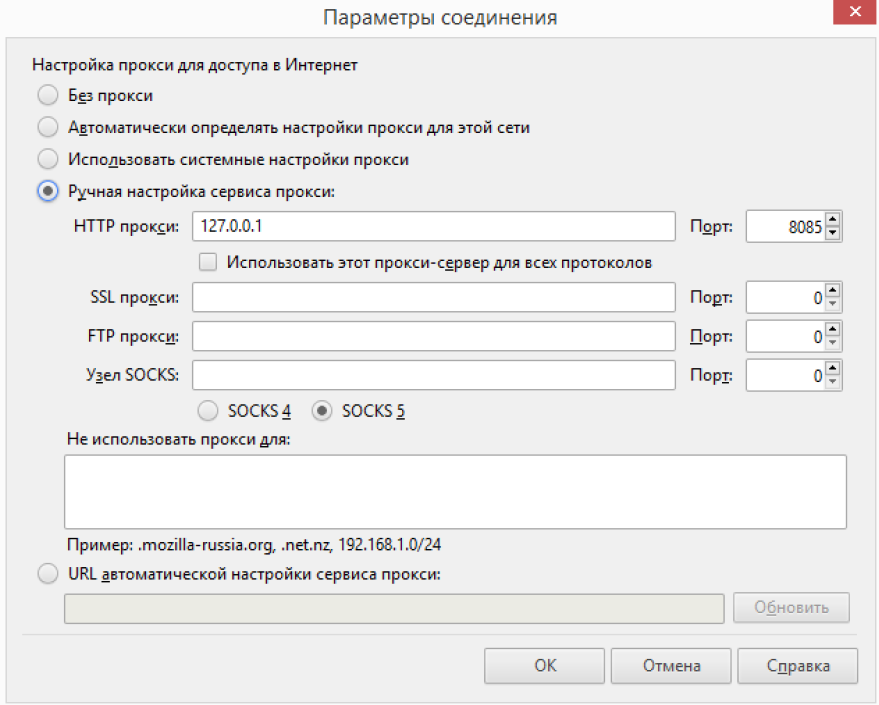
\includegraphics[scale=0.5]{2}
\caption{Настройка прокси-сервера}
\end{figure}
\FloatBarrier
Запустим ZAP и видим, что на панели сайтов появился WebGoat и перехват запросов(рисунок3).
\FloatBarrier
\begin{figure}[h!]
\centering
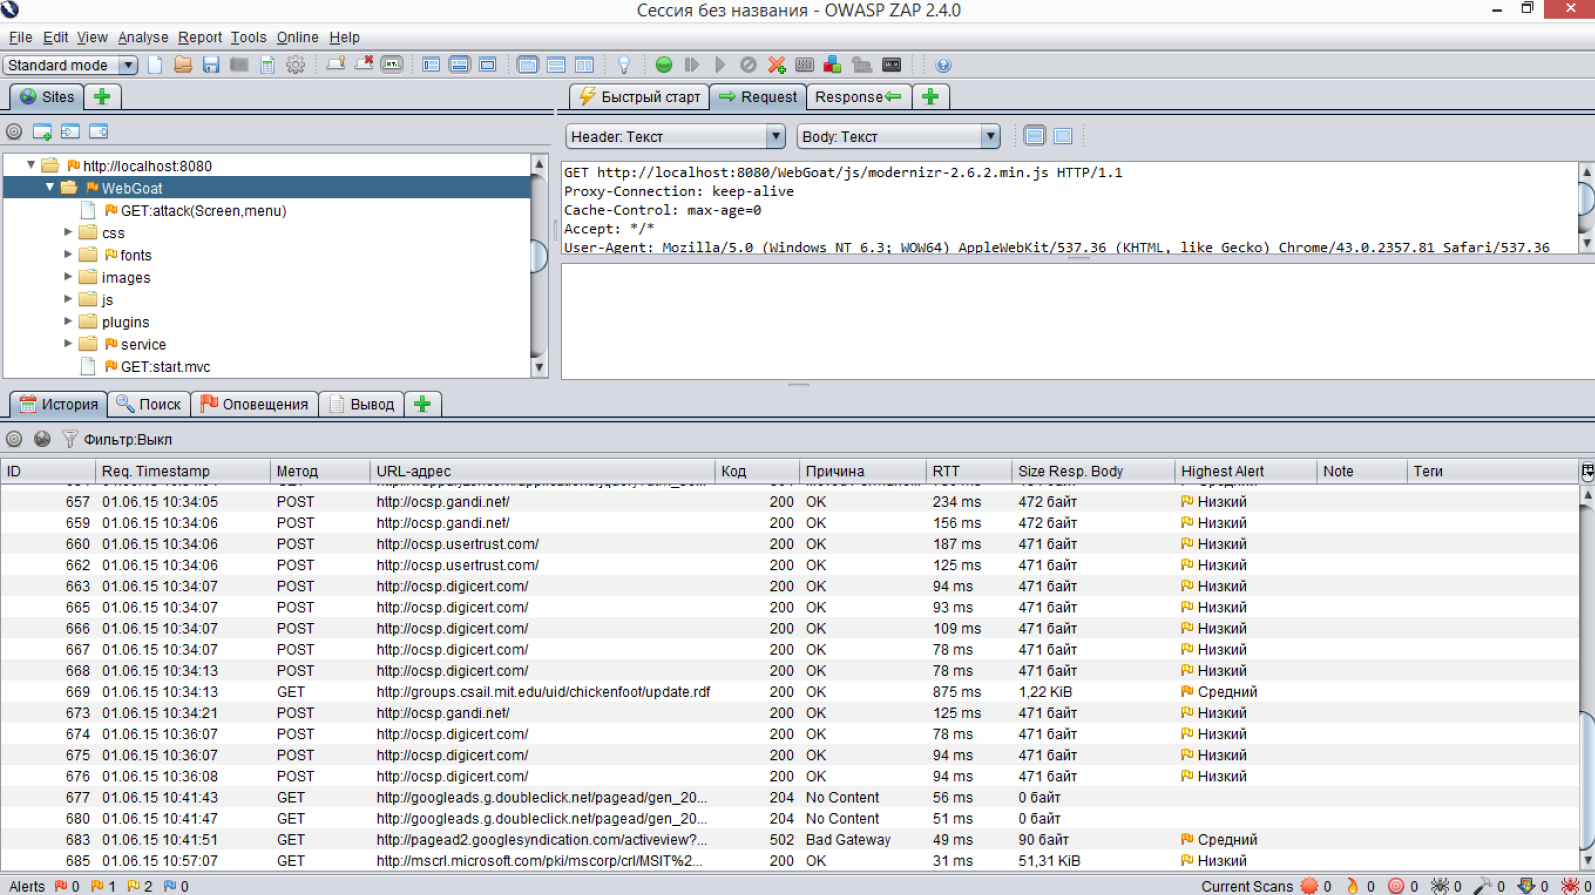
\includegraphics[scale=0.4]{3}
\caption{Работа ZAP}
\end{figure}
\FloatBarrier
Зададим Http Basics, введем своем имя в поле и поставим ZAP в режим прослушивания (рисунок 4).
\FloatBarrier
\begin{figure}[h!]
\centering
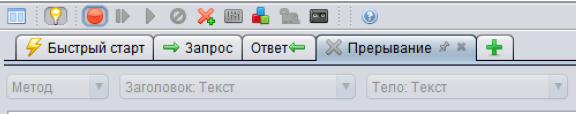
\includegraphics[scale=0.4]{4}
\caption{ZAP в режиме прослушивания}
\end{figure}
\FloatBarrier
Отправим данные (GO!) и увидим, что был перехвачем POST запрос (рисунок 5.)
\FloatBarrier
\begin{figure}[h!]
\centering
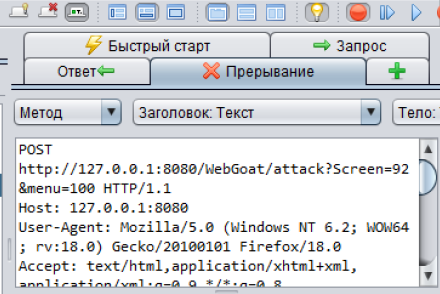
\includegraphics[scale=0.4]{5}
\caption{ZAP перехватил POST запрос}
\end{figure}
\FloatBarrier
\end{document}